\documentclass[journal]{IEEEtran}
\IEEEoverridecommandlockouts

\usepackage{cite}
\usepackage{url}
\usepackage{amsmath,amssymb,amsfonts}
\usepackage{algorithmic}
\usepackage{graphicx}
\usepackage{textcomp}
\usepackage{xcolor}
\usepackage{booktabs}
\usepackage{multirow}
\usepackage{siunitx}
\usepackage{bm}
\usepackage{gensymb}
\usepackage{tikz}
\usetikzlibrary{arrows.meta, positioning, shapes.geometric, fit, backgrounds}

\def\BibTeX{{\rm B\kern-.05em{\sc i\kern-.025em b}\kern-.08em
    T\kern-.1667em\lower.7ex\hbox{E}\kern-.125emX}}

% Math shortcuts
\newcommand{\vR}{\mathbf{R}}
\newcommand{\vp}{\mathbf{p}}
\newcommand{\vv}{\mathbf{v}}
\newcommand{\va}{\mathbf{a}}
\newcommand{\vom}{\boldsymbol{\omega}}
\newcommand{\vg}{\mathbf{g}}
\newcommand{\vu}{\hat{\mathbf{u}}}
\newcommand{\vb}{\mathbf{b}}
\newcommand{\vz}{\mathbf{z}}
\newcommand{\vOm}{\boldsymbol{\Omega}}
\newcommand{\SO}{\mathrm{SO}(3)}
\newcommand{\so}{\mathfrak{so}(3)}
\newcommand{\Exp}{\mathrm{Exp}}
\newcommand{\Log}{\mathrm{Log}}
\newcommand{\calX}{\mathcal{X}}

\begin{document}

\title{Continuous-Time Radar-Inertial Odometry\\with B-Spline Sliding Window Optimization}

\author{Timo~Weiss%
\thanks{Manuscript received Month~XX,~2026; revised Month~XX,~2026.}%
\thanks{T.~Weiss is with the Department of Informatics, Technical
University of Munich (TUM), 80333 Munich, Germany (e-mail:
timo.weiss@tum.de).}%
\thanks{Code and datasets are available at
\protect\url{https://github.com/Dr1zz3l/radar-iwr6843-driver}.}}

\markboth{IEEE Transactions on Robotics,~Vol.~XX, No.~X, Month~2026}%
{Weiss: Continuous-Time Radar-Inertial Odometry with B-Spline Sliding Window Optimization}

\maketitle

%------------------------------------------------------------------
\begin{abstract}
We present a radar-inertial odometry (RIO) system for 6-DOF state
estimation on a quadrotor using a single-chip 60\,GHz mmWave radar
(10--60 points per frame) and a 1\,kHz IMU, evaluated through aggressive
racing and attitude-tumbling flight up to \SI{10}{\radian\per\second}
--- a regime existing RIO evaluations do not cover, where the radar
model itself degrades.  The trajectory is a continuous-time quintic
position B-spline and a cumulative SO(3) orientation B-spline, optimized
by a fixed-lag smoother with Schur complement marginalization at a
0.3\,s stride over a 3\,s window; a sensor-only pipeline initializes it
without external \emph{pose} reference.  Doppler measures velocity
directly, so we evaluate RIO as a \emph{velocity and orientation}
source, reporting position as drift per distance.  A Markov-blanket
factor-selection rule makes the marginalization a true marginal, and a
single dynamics-adaptive measurement-weighting law covers hover to
\SI{10}{\radian\per\second}, validated on held-out flights.  At the live
leading edge, velocity and orientation RMSE stay below
\SI{0.5}{\metre\per\second} and \SI{3}{\degree} across racing (position
drift under \SI{1}{\percent}) and degrade gracefully to
\SI{2.9}{\percent}/\SI{6.3}{\degree} under tumbling; the output
orientation covariance is NEES-consistent.  We also document negative
results: a diagnostic for marginalization inconsistency, and that the
tumbling elevation bias is a flight-regime proxy, not an antenna
constant.
\end{abstract}

\begin{IEEEkeywords}
radar-inertial odometry, continuous-time estimation, B-spline,
sliding window, marginalization, mmWave radar, Doppler velocity
\end{IEEEkeywords}

%==================================================================
\section{Introduction}
\label{sec:intro}

Visual odometry and LiDAR-based SLAM are well-established, but both
degrade in dusty, foggy, featureless, or textureless environments.
Millimeter-wave (mmWave) FMCW radar is inherently robust to these
conditions: it penetrates smoke and dust, operates in the dark, and
measures Doppler velocity directly without feature matching.  These
properties make it attractive for aggressive flight in unstructured
environments.

Combining a mmWave radar with an IMU (RIO) for ego-motion estimation
has been explored with discrete-time EKF and graph-optimization
formulations~\cite{doer2020ekf,kramer2020rve}.  However, the
asynchronous nature of radar-IMU data (radar at $\sim$11\,Hz, IMU at
$\sim$1\,kHz) motivates a continuous-time representation where the
trajectory is a smooth function evaluated at any sensor timestamp
without interpolation approximation.

\textbf{Research question.}
This work asks, end to end: \emph{can a single-chip mmWave radar,
fused with an IMU, provide usable 6-DOF state estimation --- and if
so, what does it take to obtain good results?}  The answer is
structured in three parts.  (1)~\emph{What the sensor provides:}
per-point Doppler yields direct ego-velocity, but at 10--60 points
per frame there are no bearing-stable features for position fixing;
yaw is a gauge freedom of Doppler+IMU.  The system is therefore a
\emph{velocity and orientation} source whose position estimate drifts
with distance --- by construction, not by defect.  (2)~\emph{What it
takes:} a consistent fixed-lag smoother and a dynamics-adaptive
weighting of every measurement stream, each step of which we derive
from a measured failure diagnosis rather than tuning folklore.
(3)~\emph{What the limits are:} characterized via held-out flights,
extreme maneuvers, calibrated output covariance, and documented
negative results.

We contribute:
\begin{itemize}
  \item \emph{Single-chip radar under aggressive and tumbling flight},
        characterizing how the radar measurement model breaks in this
        regime: rate-dependent intra-frame smearing, and the finding
        that the apparent elevation bias under tumbling is a
        flight-regime error proxy, not a physical antenna constant.
        Backflips at \SI{10}{\radian\per\second} on a single-chip
        sensor are, to our knowledge, unexplored.
  \item A \emph{consistency-analyzed} fixed-lag smoother: a factor-set
        selection rule exploiting B-spline local support to make the
        Schur marginal exactly closed --- distinct from and
        complementary to FEJ --- eliminating prior-weight tuning, at
        0.35--0.70\,s per window on a laptop (real time for aggressive
        racing).
  \item One measurement-weighting configuration from hover to
        \SI{10}{\radian\per\second}, with the velocity--orientation
        trade as a measured Pareto curve and accuracy validated on
        \emph{held-out flights} never used for tuning.
  \item Honest negative results: a diagnostic symptom pattern for
        marginalization inconsistency; a representation-level study
        that \emph{disproves} the adaptive-knot-density hypothesis for
        this regime; ground-truth limits during aggressive maneuvers;
        and a NEES check confirming the reported orientation covariance
        is consistent on racing flights.
\end{itemize}
The complete system --- physically correct Doppler model with lever
arm, sensor-only initialization, full hyperparameter disclosure,
deterministic re-runs --- is released with code and datasets for
independent reproduction.

\textbf{Data and code.}
The datasets (Vicon MoCap lab, TI IWR6843AOPEVM, Pixhawk) and the
C++ Ceres solver with Python bindings used in this work are available
at \url{https://github.com/Dr1zz3l/radar-iwr6843-driver}.

%==================================================================
\section{Related Work}
\label{sec:related}

\textbf{Radar ego-velocity estimation.}
Doppler-based ego-velocity estimation from mmWave radar was
demonstrated by Kellner et al.~\cite{kellner2014instantaneous} and
extended to 3D with weighted least squares by
Kramer et al.~\cite{kramer2020rve}, whose RVE system fuses radar
with IMU in a discrete-time EKF.  Doer et
al.~\cite{doer2020ekf} present an EKF-based RIO with online
extrinsic calibration. Our work uses the same per-frame WLS
ego-velocity estimator but embeds it in a continuous-time
batch/sliding-window optimizer.

\textbf{Continuous-time trajectory estimation.}
Furgale et al.~\cite{furgale2013unified} introduced uniform B-splines
for continuous-time visual-inertial calibration.  The basalt
VIO~\cite{usenko2020basalt} uses cumulative B-splines on Lie groups
for stereo-inertial odometry. We adapt the basalt-style cumulative
SO(3) B-spline to radar-inertial fusion.

\textbf{Marginalization in sliding-window estimators.}
OKVIS~\cite{leutenegger2015keyframe} and
VINS-Mono~\cite{qin2018vins} pioneered Schur complement
marginalization for visual-inertial systems, propagating information
from dropped keyframes as a dense Gaussian prior. We apply the same
principle to continuous-time B-spline control points and document
the practical challenges of prior scaling when information asymmetry
spans ten orders of magnitude.

\textbf{Closest related work.}
Continuous-time radar-inertial odometry was introduced by
Ng et al.~\cite{ng2021ctrio}, who fuse Doppler measurements from
\emph{multiple automotive} radars with an IMU as a least-squares
problem over a B-spline trajectory, evaluated on passenger vehicles.
Burnett et al.~\cite{burnett2024gp} use a Gaussian-process motion
prior for spinning-radar- and lidar-inertial odometry, and
\v{S}tironja et al.~\cite{stironja2026rio} model the IMU trajectory
continuously inside an RIO estimator with online spatio-temporal
calibration.  Single-chip radar-inertial estimation has itself
received recent attention --- Huang et al.~\cite{huang2024lessismore}
exploit radar cross-section and Doppler physics to make a sparse
single-chip cloud usable, in a discrete-time sliding-window
optimization --- but on ground-robot and handheld platforms rather
than aerial tumbling flight.
Our setting differs from all of these in sensor and
regime: a \emph{single-chip} radar (10--60 points per frame,
2-TX elevation array) on a quadrotor in aggressive racing and
attitude-tumbling flight up to \SI{10}{\radian\per\second} --- a
regime in which, as Sec.~\ref{sec:backflips} shows, the radar
measurement model itself degrades in ways invisible on ground
vehicles.

\textbf{Sliding-window marginalization and consistency.}
That na\"ive sliding-window marginalization is inconsistent is long
established in discrete time: Dong-Si and
Mourikis~\cite{dongsi2012consistency} analyze which retained states
may legitimately connect to marginalized ones, and first-estimates
Jacobian (FEJ) methods fix linearization points to preserve the
observability nullspace.  In continuous time,
CLIC~\cite{lv2023clic} and
LIO-MARS~\cite{quenzel2025liomars} marginalize spline knots leaving
the window, and Hug et al.~\cite{hug2022continuous} apply Schur
marginalization to visual-inertial splines.  Our contribution to this
line is narrower and complementary to FEJ: a factor-\emph{set}
selection rule that exploits B-spline local support to make the
marginal exactly closed (no double counting, no conditioning on
interior states), and a documented symptom pattern by which the
inconsistent variant can be recognized (Sec.~\ref{sec:prior_scale}).
In the discrete-time UAV line, Doer and
Trommer~\cite{doer2020ekf} and 4D-radar-aided inertial
navigation define the state of practice.
Rather than comparing numbers across papers --- our own quantization
ablation (Sec.~\ref{sec:heldout}) shows firmware configuration alone
changes Doppler resolution by $12\times$ --- we cross-validate against
this line directly: Sec.~\ref{sec:baselines} runs our system on the
public ICINS-2021 flight datasets of~\cite{doer2021yrio} and re-evaluates
their EKF estimators under our causal metrics on the same data, and
reports the regime-dependent result of porting their filters to our
platform.

%==================================================================
\section{System Overview}
\label{sec:overview}

\subsection{Hardware Platform}
The system runs on a quadrotor with a TI IWR6843AOPEVM
mmWave radar (60--64\,GHz FMCW), a Pixhawk flight
controller IMU, and a Vicon MoCap system used for ground
truth evaluation.  The radar is mounted upside-down with a nominal
$30\degree$ downward tilt (CAD); the mount is 3D-printed and
hand-assembled, so the as-built angle is uncertain by a few degrees and
is recovered by online extrinsic calibration (Sec.~\ref{sec:results}).
The nominal extrinsic rotation is $[180\degree, 25.5\degree, 0\degree]$
(roll, pitch, yaw), translation $[0.08, 0.02, -0.01]$\,m in the body
frame.  The radar operates at $\sim$11\,Hz with 0.049\,m/s Doppler
resolution (best-velocity firmware configuration).  Raw IMU rate
is $\sim$993\,Hz; both modalities are used at full rate.

\subsection{Pipeline}
Fig.~\ref{fig:pipeline} shows the three-stage initialization feeding
into a C++ Ceres solver (batch or sliding window):
\textbf{P1} derives initial roll/pitch from the stationary
accelerometer and forward-integrates gyroscope measurements;
\textbf{P2} estimates per-frame ego-velocity with WLS and integrates
to a position trajectory;
\textbf{P3} builds sensor-only boundary priors at $t=0$.
MoCap data is loaded only for final RMSE evaluation.

\begin{figure}[t]
\centering
\scalebox{0.92}{%
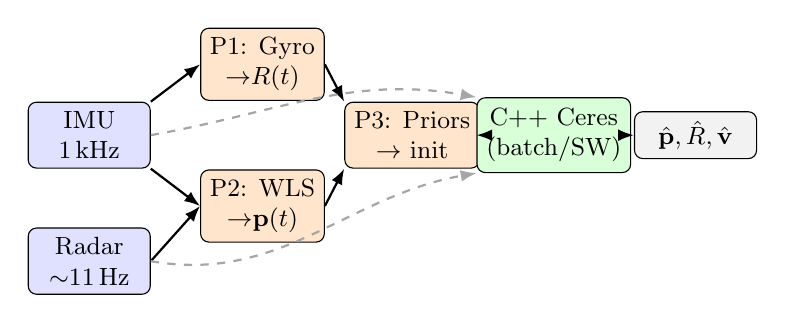
\begin{tikzpicture}[
  font=\small,
  box/.style={rectangle, rounded corners=3pt, draw, minimum width=1.55cm,
              minimum height=0.52cm, align=center},
  sensor/.style={box, fill=blue!12},
  stage/.style={box, fill=orange!20},
  solver/.style={box, fill=green!15, minimum width=1.6cm, minimum height=0.95cm},
  arr/.style={-{Latex[length=2mm]}, thick},
  darr/.style={-{Latex[length=2mm]}, thick, dashed, gray!70},
  ]
  %% Nodes: sensor column, two init stages, merge/P3 stage, solver, output
  \node[sensor] (imu)    at (0.0,  1.1) {IMU\\1\,kHz};
  \node[sensor] (radar)  at (0.0, -0.5) {Radar\\$\sim$11\,Hz};
  \node[stage]  (p1)     at (2.2,  2.0) {P1: Gyro\\${\to}R(t)$};
  \node[stage]  (p2)     at (2.2,  0.2) {P2: WLS\\${\to}\mathbf{p}(t)$};
  \node[stage]  (p3)     at (4.1,  1.1) {P3: Priors\\${\to}$ init};
  \node[solver] (solver) at (5.9,  1.1) {C++ Ceres\\(batch/SW)};
  \node[box, fill=gray!10] (out) at (7.7, 1.1)
        {$\hat{\mathbf{p}},\hat{R},\hat{\mathbf{v}}$};

  %% Init pipeline arrows (solid, no crossings by construction)
  % IMU → P1 (upper-right diagonal)
  \draw[arr] (imu.north east) -- (p1.west);
  % IMU → P2 (lower-right diagonal; meets Radar→P2 at P2, no earlier crossing)
  \draw[arr] (imu.south east) -- (p2.west);
  % Radar → P2 (upper-right; both end at P2 → no crossing)
  \draw[arr] (radar.east)     -- (p2.west);
  % P1 and P2 → P3 (converge; meet at P3, no earlier crossing)
  \draw[arr] (p1.east)        -- (p3.north west);
  \draw[arr] (p2.east)        -- (p3.south west);
  % P3 → Solver
  \draw[arr] (p3.east)        -- (solver.west);
  % Solver → Output
  \draw[arr] (solver.east)    -- (out.west);

  %% Raw-data feeds (dashed, routed above/below init block to avoid crossings)
  \draw[darr] (imu.east)   to[out=10,  in=170] (solver.north west);
  \draw[darr] (radar.east) to[out=350, in=190] (solver.south west);
\end{tikzpicture}%
}% end scalebox
\caption{System pipeline. Solid: initialization flow (P1--P3 seed
the optimizer). Dashed: raw sensor data fed as measurement factors.
Radar returns first pass a RANSAC ego-velocity prefilter
(Sec.~\ref{sec:models}) that rejects elevation-biased outliers before
both P2 and the solver. MoCap used only for RMSE evaluation.}
\label{fig:pipeline}
\end{figure}

%==================================================================
\section{Methodology}
\label{sec:method}

\subsection{State Representation}
\label{sec:state}

\textbf{Position.}
The world-frame position $\vp_w(t) \in \mathbb{R}^3$ is a quintic
(order-6) uniform B-spline with knot spacing $\Delta t_p = 5$\,ms.
Velocity $\dot{\vp}_w$ and acceleration $\ddot{\vp}_w$ are
obtained as analytical derivatives of the spline.

\textbf{Orientation.}
We use the \emph{cumulative} SO(3) B-spline
formulation~\cite{sommer2020efficient}:
\begin{equation}
  \vR(t) = \vR_{\mathrm{base}}[k{-}3]
           \prod_{j=k-3}^{k} \Exp\!\bigl(\tilde{B}_j(t)\,\vOm_j\bigr),
  \label{eq:ori_spline}
\end{equation}
where $k$ is the active knot index for time $t$,
$\vOm_j \in \so$ are incremental rotation control points
(standard $\Exp$/$\Log$ map convention),
$\tilde{B}_j(t)$ are cumulative cubic basis functions, and
$\vR_{\mathrm{base}}$ is the left anchor rotation.  Knot spacing
is $\Delta t_o = 8$\,ms.  Body-frame angular velocity $\vom_b(t)$
is obtained as a closed-form derivative of~\eqref{eq:ori_spline}
directly from \texttt{evaluate\_lie()} without numerical
differentiation.

\textbf{Biases and extrinsics.}
A constant 6-DoF IMU bias $[\vb_a, \vb_g]$ is estimated jointly.
The extrinsic pitch $\delta_\text{pitch}$ (1 DoF) is optimized
with a soft prior; roll and yaw are fixed (unobservable from
Doppler).  It is optimized in batch for self-calibration and locked at
the calibrated 27.5\degree\ for the sliding window
(Sec.~\ref{sec:backflips}).

\subsection{Measurement Models}
\label{sec:models}

\textbf{Radar Doppler with lever arm.}
The TI IWR6843 reports positive Doppler for a receding target.
With antenna offset $\mathbf{t}_{bs}$ from the body CoM, the
predicted Doppler for a point at sensor-frame bearing $\vu_s$ is:
\begin{equation}
  v_D = -\vu_b^{\top}\!\left(
    \vR_{bw}\,\vv_w(t) + \vom_b(t) \times \mathbf{t}_{bs}
  \right),
  \label{eq:doppler}
\end{equation}
where $\vu_b = \vR_{bs}\,\vu_s$, $\vR_{bs}$ is the rotation from
radar sensor to body frame (extrinsic $[\text{roll}{=}180\degree,\,
\text{pitch}{=}25.5\degree,\,\text{yaw}{=}0\degree]$), and
$\vR_{bw} = \vR_{wb}^{\top}$.  The residual
$r_k = v_{D,\text{meas}} - v_{D,\text{pred}}$ uses Huber
loss with $\delta = 1.0$\,m/s --- robust, as defense-in-depth, to any
residual Doppler noise on the surviving inlier returns; the
\SI{0.049}{\metre\per\second} Doppler resolution sets a lower bound but
does not drive the choice.

\textbf{RANSAC ego-velocity prefilter (default front-end).}
A single-chip radar with only 2\,TX antennas has limited elevation
diversity, and a minority of returns carry an elevation-correlated
Doppler bias that a robust kernel only down-weights.  Following
reve~\cite{doer2020ekf}, we therefore prepend a reve-style 3D
least-squares RANSAC ego-velocity estimate to the per-frame Doppler set
(inlier threshold $0.15$\,m/s) and pass only the inlier returns to the
spline solver, hard-rejecting the elevation-biased minority before the
optimization.  The prefilter is seeded
(\texttt{numpy.default\_rng(0)}), so the full pipeline reproduces
bit-identically; frames with fewer than five returns bypass it
unchanged --- on those sparse frames, including most of the backflip
regime, the in-solver Huber loss is the sole radar outlier protection,
so the two stages are complementary, not redundant.  It runs once at
frame load, not per window, so it does not
enter the per-window timing budget (Sec.~\ref{sec:results}).
Sec.~\ref{sec:baselines} quantifies what it removes --- on the public
ICINS flights it closes an order-of-magnitude vertical-drift gap, and on
our own flights it improves aggressive-racing live position by $22\%$ ($0.50\to0.39$\,m
live) --- and it is enabled by default for every result in this paper.

\textbf{Dynamics-adaptive measurement weighting.}
The central practical finding of this work is that a single
\emph{rate-adaptive trust allocation} across the three measurement
streams covers hover to \SI{10}{\radian\per\second} tumbling with one
configuration.  Each component was derived from a measured failure
diagnosis (Sec.~\ref{sec:backflips}), not tuned ad hoc:
\begin{itemize}
\item \emph{Gyroscope --- trust more when rotating fast.}
  Per-sample weight
  $\lambda_g^{\mathrm{eff}} = \lambda_g\bigl(1 + (|\vz_g|/\omega_g)^p\bigr)$
  with $\lambda_g{=}4$, $\omega_g{=}4$\,rad/s, $p{=}4$, using the
  \emph{measured} rate (causal, no spline evaluation).  The quartic
  exponent keeps racing untouched ($\lambda^{\mathrm{eff}}\!\approx\!\lambda_g$
  below 3\,rad/s) and reaches $\lambda^{\mathrm{eff}}\!\approx\!160$--$500$
  during flips, where the gyroscope is the only clean sensor.  A
  quadratic ramp ($p{=}2$) stiffens the gyro already at 2--5\,rad/s ---
  where radar is still informative --- and degrades racing roll/yaw.
\item \emph{Radar --- trust less when rotating fast.}
  A radar frame integrates over tens of milliseconds; at body rate
  $\omega$ the scene smears by $\omega\,T_{\mathrm{frame}}$
  ($\approx$17\degree\ at 10\,rad/s).  Per-frame noise inflation
  $\sigma_{\mathrm{eff}}^2 = \sigma_0^2\bigl(1+(|\vom|/\omega_r)^2\bigr)$,
  $\omega_r{=}4$\,rad/s, $|\vom|$ from the warm-start spline at
  problem-build time; continuous, no hard-gate tuning cliff.
\item \emph{Accelerometer --- same form,} $\omega_a{=}8$\,rad/s:
  during flips the accelerometer carries thrust transients and
  vibration, its gravity information is nil mid-flip, and it otherwise
  distorts orientation through the $\vR$--$\ddot{\vp}$ coupling.
\item \emph{Per-point SNR weighting.}
  $w_i = \mathrm{clip}\bigl((I_i/\tilde{I})^{\alpha},\,0.25,\,4\bigr)$
  with frame-median intensity $\tilde I$ and $\alpha{=}1$
  (median-relative, so the global radar weight is unchanged).  High-SNR
  returns carry measurably better Doppler: on aggressive racing this
  alone improves live orientation from 3.31\degree\ to 2.88\degree\ at
  unchanged position.
\end{itemize}
The weighting trades are made explicit in
Sec.~\ref{sec:backflips}: on tumbling flight the radar/accelerometer
gates exchange velocity accuracy for orientation accuracy along a
measured Pareto curve; $(\omega_r,\omega_a){=}(4,8)$ is its knee.

\textbf{Flip-regime Doppler correction.}
Under sustained tumbling an additional attitude-correlated Doppler
systematic appears, which we absorb with a per-point term
$v_{\mathrm{corr}} = v_{\mathrm{meas}} - b\,u_{s,z}$ ($b{=}{-}1.5$\,m/s,
backflips only).  Sec.~\ref{sec:backflips} shows why $b$ must be
interpreted as a flight-regime error proxy rather than a physical
elevation bias of the 2-TX array.

\textbf{Accelerometer.}
\begin{equation}
  \mathbf{r}_a = \vz_a - \vR_{bw}\!\left(\ddot{\vp}_w - \vg_w\right) - \vb_a,
  \label{eq:accel}
\end{equation}
weighted $\lambda_a = 0.01$.

\textbf{Gyroscope.}
\begin{equation}
  \mathbf{r}_g = \vz_g - \vom_b(t) - \vb_g,
  \label{eq:gyro}
\end{equation}
weighted $\lambda_g = 4.0$ (L2 loss).

\textbf{Gravity direction.}
\begin{equation}
  \mathbf{r}_{\mathrm{tilt}} =
    \frac{\vz_a - \vb_a}{\|\vz_a - \vb_a\|} - \vR_{bw}^{\top}\hat{\vg},
  \label{eq:tilt}
\end{equation}
active when $\bigl|\,\|\vz_a{-}\vb_a\| - g\,\bigr| < 3\,\mathrm{m/s}^2$.
This provides roll/pitch anchoring during near-hover phases without
contaminating dynamic flight.

\textbf{Heading prior.}
Yaw is unobservable from Doppler alone (all yaw-equivalent
trajectories predict identical radial velocities under pure
rotation about gravity).  We supply a heading reference from a magnetometer (standard on
most platforms; here simulated by MoCap yaw).  The residual $r_\psi = \psi_\text{est} - \psi_\text{ref}$
is added at $\sim$100\,Hz, with $\lambda_\psi = 0.6$ by default and
raised to $10$ on the heading-critical bags (slow racing, backflips;
Table~\ref{tab:sw} footnote).

\subsection{Regularization}
\label{sec:reg}

\textbf{Position: minimum snap.}
$E_{\text{snap}} = \lambda_s \int \|\vp^{(4)}(t)\|^2\,dt$
with $\lambda_s = 2{\times}10^{-5}$.

\textbf{Orientation: minimum angular acceleration.}
Rather than penalizing angular velocity increments (minimum $\omega$),
which opposes every banked turn and the entire backflip maneuver, we
penalize the \emph{second} finite difference on SO(3):
\begin{equation}
  \mathbf{r}_\alpha = \Log(\vR_{i-1}^{-1}\vR_i)
                    - \Log(\vR_i^{-1}\vR_{i+1}),
  \label{eq:min_alpha}
\end{equation}
which is zero for constant angular rate.
Swept $\lambda_\alpha \in \{0, 0.001, 0.01, 0.1, 1.0\}$; 0.1
was best across all bags (1.0 caused backflip divergence).

\subsection{Sensor-Only Initialization (P1--P3)}
\label{sec:init}

\textbf{P1: Orientation.}
A stationary segment before flight is detected automatically; the IMU
biases $[\vb_a, \vb_g]$ are seeded from the gravity residual and mean
gyroscope reading during this segment (MoCap orientation is used for a
full 3-D accelerometer bias estimate when available; otherwise a gravity-
aligned scalar correction is applied).
Initial roll/pitch are then derived from the stationary accelerometer
(gravity direction).  Yaw is set to zero (gauge freedom; corrected
later by the heading prior).  The full orientation trajectory is
obtained by forward-integrating debiased gyroscope readings:
$\vR(t+\Delta t) = \vR(t)\,\Exp\!\bigl((\vz_g - \vb_g)\Delta t\bigr)$.

\textbf{P2: Position.}
Per radar frame, weighted least squares estimates the 3D ego-velocity
$\vv_{\text{wls}}$ from the RANSAC inlier returns
(Sec.~\ref{sec:models}).  Doppler alias
unwrapping uses IMU-integrated world-frame velocity to select the
correct alias before the main solver runs (20.9\% of points aliased
in fast racing, 1.7\% in slow racing).
World-frame velocity is integrated with forward Euler to produce an
initial position trajectory.

\textbf{P3: Boundary priors.}
Position, velocity, orientation, and angular velocity boundary
priors are built from the sensor-only state at $t=0$.
$\lambda_{\text{bnd}} = 1000$ for position and velocity.

\subsection{Sliding Window with Schur Complement Marginalization}
\label{sec:sw}

\begin{figure}[t]
\centering
\scalebox{0.97}{%
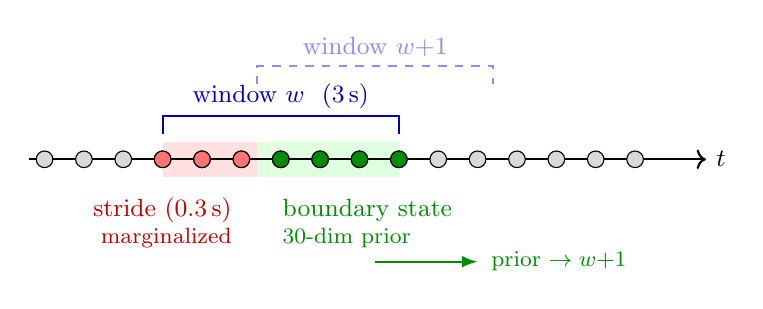
\begin{tikzpicture}[
  font=\small,
  cp/.style={circle, draw, minimum size=6pt, inner sep=0pt},
  ]
  % --- shaded zone backgrounds (draw first, CPs on top) ---
  \fill[red!12]   (1.5,-0.22) rectangle (2.7, 0.22);
  \fill[green!12] (2.7,-0.22) rectangle (4.5, 0.22);

  % --- timeline ---
  \draw[->, thick] (-0.2,0) -- (8.4,0) node[right]{$t$};

  % --- gray CPs ---
  \foreach \x in {0.0, 0.5, 1.0, 1.5, 2.0, 2.5, 3.0, 3.5, 4.0,
                  4.5, 5.0, 5.5, 6.0, 6.5, 7.0, 7.5}
    \node[cp, fill=gray!30] at (\x, 0) {};

  % --- red (marginalized) CPs ---
  \foreach \x in {1.5, 2.0, 2.5}
    \node[cp, fill=red!55] at (\x, 0) {};

  % --- green (boundary) CPs ---
  \foreach \x in {3.0, 3.5, 4.0, 4.5}
    \node[cp, fill=green!55!black] at (\x, 0) {};

  % === ABOVE the timeline: window span brackets ===

  % Window w bracket: ticks at y=0.32, horizontal bar at y=0.55, label at y=0.75
  \draw[blue!75!black, thick]
    (1.5,0.32) -- (1.5,0.55) -- (4.5,0.55) -- (4.5,0.32);
  \node[blue!75!black] at (3.0, 0.80) {window $w$ \ (3\,s)};

  % Window w+1 bracket: ticks at y=0.95, bar at y=1.18, label at y=1.38
  \draw[blue!45, thick, dashed]
    (2.7,0.95) -- (2.7,1.18) -- (5.7,1.18) -- (5.7,0.95);
  \node[blue!45] at (4.2, 1.43) {window $w{+}1$};

  % === BELOW the timeline: zone labels ===
  % Red anchored east (text grows left); green anchored west (text grows right)
  % → labels always point away from the shared boundary at x=2.7

  \node[red!75!black, anchor=east] at (2.5, -0.65) {stride (0.3\,s)};
  \node[red!75!black, anchor=east, font=\footnotesize] at (2.5, -1.00) {marginalized};

  \node[green!55!black, anchor=west] at (2.9, -0.65) {boundary state};
  \node[green!55!black, anchor=west, font=\footnotesize] at (2.9, -1.00) {30-dim prior};

  % Prior propagation: boundary CPs feed the next window
  \draw[-{Latex[length=2mm]}, green!55!black, thick]
    (4.2, -1.30) to[out=0, in=180] (5.5, -1.30);
  \node[green!55!black, font=\footnotesize, anchor=west] at (5.55, -1.30)
    {prior $\to w{+}1$};

\end{tikzpicture}%
}% end scalebox
\caption{Sliding window: red CPs (stride zone) are marginalized
into a 30-dim Gaussian prior on the green boundary CPs.}
\label{fig:sw_diagram}
\end{figure}

The fixed-lag smoother advances a 3\,s window in 0.3\,s strides.
After each Ceres LM solve, the \emph{stride zone} CPs and orientation
knots are marginalized:
\begin{equation}
  S = H_{bb} - H_{ab}^{\top} H_{aa}^{-1} H_{ab},
  \label{eq:schur}
\end{equation}
where $a$ indexes stride-zone variables and $b$ indexes boundary
variables (last $N{-}1$ position CPs, last $N{-}1$ orientation
knots, and the 6-DoF bias; dimension 30).  $S$ is factored as
$S = LL^{\top}$ and stored as a \texttt{MargPriorFunctor} for the
next window.

\textbf{Re-centered prior.}
Before adding the prior to each window's problem, the linearization
point $\mathbf{x}_0$ is updated to the current warm-start.  This
makes the prior contribute only curvature (the Hessian shape), not a
gradient pull toward a stale historical estimate.  The residual is
$\mathbf{r} = L^{\top}(\mathbf{x} - \mathbf{x}_0)$ in local
coordinates.

\textbf{Consistent factor selection (Markov-blanket rule).}
Which residuals enter Eq.~\eqref{eq:schur} determines whether the
prior is a true marginal.  A na\"ive choice --- all residuals touching
marginalized \emph{or} boundary variables --- pulls in every IMU factor
of the window through the shared bias block ($\sim$25{,}000 residual
rows), \emph{conditions} on interior states (treating them as perfectly
known), and double-counts factors that are re-added in the next window.
The resulting prior is overconfident by orders of magnitude and must be
deflated by a hand-tuned scale of $10^{-7}$--$2{\times}10^{-4}$
depending on flight dynamics (Sec.~\ref{sec:prior_scale}).
We instead exploit B-spline locality: a factor touching marginalized
knot $i$ has support $[i, i{+}N{-}1] \subseteq$
marg\,$\cup$\,boundary, so including \emph{only} residuals that touch a
marginalized variable (plus the previous prior) yields an exactly
closed, consistent marginal.  With this rule the prior is applied
\textbf{unscaled} (scale $=1$) across all flight regimes, and its
Mahalanobis residual at the solution drops from $10^{6}$--$10^{12}$
to $\mathcal{O}(1)$ --- the prior agrees with the incoming data.

\emph{Relation to FEJ.}  This mechanism is distinct from, and
complementary to, first-estimates-Jacobian approaches to
marginalization consistency~\cite{dongsi2012consistency}: FEJ fixes
the \emph{linearization points} of the prior to preserve the
observability nullspace, whereas our rule corrects the
\emph{factor set} entering the Schur complement so that the marginal
is exactly closed \emph{at a fixed linearization point}.  We do not
employ FEJ; instead the prior is re-centered at each window's warm
start (curvature retained, gradient pull discarded).  We do not claim
this re-centering preserves consistency across relinearizations as a
theoretical guarantee; rather, in our experiments it left no measurable
inconsistency symptom --- the NEES analysis of
Sec.~\ref{sec:nees} provides the corresponding empirical evidence.

\textbf{Live-edge warm start.}
Control points entering the window each stride would otherwise hold
stale dead-reckoned initialization values; any CP-level seam is
amplified by the min-snap term ($\propto \Delta/\Delta t_p^4$, initial
cost $\sim$$10^{13}$).  We rigidly align the entering segment (shift +
$\Delta R$) to the last data-supported CP of the previous solution,
reducing the initial cost by five orders of magnitude.

\textbf{Marginalization cost.}
The restricted Gauss--Newton Hessian for Eq.~\eqref{eq:schur} is
accumulated by evaluating the affected cost functions directly
(tangent-space Jacobians via the manifold plus-Jacobian, Triggs
correction for robust losses), avoiding a full solver re-linearization;
the marginalization step costs $\sim$10\,ms per window.

%==================================================================
\section{Experimental Setup}
\label{sec:setup}

All experiments use the rosbag datasets collected in a Vicon MoCap
lab.  Table~\ref{tab:datasets} summarizes the three bags used for
evaluation.

\begin{table}[t]
\centering
\caption{Dataset Summary}
\label{tab:datasets}
\small
\begin{tabular}{@{}lcccc@{}}
\toprule
Bag & Dur.\ (s) & $v_{\max}$ (m/s) & $|\omega|_{\max}$ (rad/s) & Frames \\
\midrule
Slow racing & 25.8 & 3.65 & 2.62 & 258 \\
Fast racing & 18.0 & 5.66 & 9.14 & 179 \\
Backflips\textsuperscript{*} & 18.1 & $\sim$4.3 (95\%) & $\sim$10.9 (95\%) & 181 \\
\bottomrule
\multicolumn{5}{l}{\textsuperscript{*}95th percentile; MoCap tracking artifacts dominate peaks.}
\end{tabular}
\end{table}

\textbf{IMU rate:} $\sim$993\,Hz (full rate, no downsampling for C++ solver).
\textbf{Evaluation:} Start-anchored rigid alignment to MoCap ground
truth: the alignment rotation $\mathbf{R}_\mathrm{align} =
\mathbf{R}_{\mathrm{gt},0}\,\mathbf{R}_{\mathrm{est},0}^\top$
and translation $\mathbf{t}_\mathrm{align} =
\mathbf{p}_{\mathrm{gt},0} - \mathbf{R}_\mathrm{align}\,
\mathbf{p}_{\mathrm{est},0}$ are fixed at frame~0 (no scale).
The final 3\,s is trimmed.  Velocity RMSE is computed from the
analytical first derivative of the position B-spline, not from finite
differences of the estimated trajectory.
\emph{Position drift} (\%) is position RMSE normalised by the total
GT path length --- the standard odometry metric for a
dead-reckoning system with no loop closure.
Start-anchored alignment is harsher than the whole-trajectory
SE(3)/Umeyama fit (the EVO/KITTI default) used by most odometry papers,
because it cannot retro-fit a constant transform to cancel accumulated
drift: it fixes the frame once, at the start, exactly as a deployed
estimator must.  We adopt it precisely for this causal,
deployment-relevant reading, and apply it identically to every system
compared.  Where we compare against externally published figures
(Sec.~\ref{sec:baselines}) we additionally report whole-trajectory-aligned
numbers so the baselines can be cross-checked against their own papers.
\emph{Translational RPE} (relative pose error, Fig.~\ref{fig:rpe}) is
the KITTI-standard per-segment displacement error averaged over all
sub-segments of a given accumulated GT length.
Because the start-anchored alignment offsets cancel within every
relative displacement, RPE is alignment-independent.
For sliding window, \emph{live (leading-edge)} RMSE is computed by
snapshotting the estimate at $[t_\text{end}{-}\text{stride},\, t_\text{end}]$
of each window at 50\,Hz before any subsequent refinement.  The
\emph{settled} RMSE evaluates the same trajectory after all windows
have refined each point.

\textbf{Solver implementation.}
The Ceres LM problem is solved with \texttt{SPARSE\_NORMAL\_CHOLESKY}
(SuiteSparse), up to 400 iterations.
All three factor types (gyroscope, accelerometer, and radar Doppler)
use hand-derived analytic Jacobians based on the basalt
cumulative-spline Jacobian struct; Ceres automatic differentiation was
eliminated to avoid Jet-arithmetic overhead over the large set of
spline control-point parameters per factor.
In the sliding-window solver the linear solve and the
marginalization-prior recompute (\texttt{compute\_prior}) are the
dominant costs; Jacobian evaluation accounts for roughly 25--30\% of
per-window wall time.

%==================================================================
\section{Results}
\label{sec:results}

\subsection{Batch Solver and Extrinsic Self-Calibration}
We use the full-trajectory C++ batch solve as the extrinsic
self-calibration stage; offline it reaches
\SI{0.20}{\metre}\,/\,\SI{1.0}{\degree} on slow racing and
\SI{0.73}{\metre}\,/\,\SI{2.5}{\degree} on fast (the dense racing
$\Delta t_p$ over-fits fast racing, where the coarser sliding window
does better).
With the extrinsic pitch left free, it self-calibrates from the
25.5\degree\ nominal to 27.0\degree\ (slow racing) and 27.2\degree\
(fast racing) --- recovering the as-built mount angle, which the
3D-printed, hand-assembled fixture leaves a few degrees short of the
30\degree\ CAD nominal.  Racing bags converge to the same pitch estimate
whether initialized at 25.5\degree\ or 30\degree, so the estimate is
data-driven, not init-dependent --- an independent check on the
extrinsic calibration.  We lock pitch at 27.5\degree\ for the
sliding-window runs (Sec.~\ref{sec:backflips}).  The batch estimate is
shown for reference (dashed red) in the trajectory overlays
(Figs.~\ref{fig:traj_slow},~\ref{fig:traj_fast}) and the RPE curves
(Fig.~\ref{fig:rpe}).

\subsection{Sliding Window: Settled vs.\ Live}
\label{sec:sw_results}

Table~\ref{tab:sw} reports sliding window results
(3\,s window, 0.3\,s stride, Schur marginalization).
Figures~\ref{fig:traj_slow} and~\ref{fig:traj_fast} show
trajectory overlays for both bags; Fig.~\ref{fig:error_time} shows
the corresponding error timeseries.

\begin{table}[t]
\centering
\caption{Sliding Window: Settled and Live Leading-Edge RMSE
  (consistent unscaled prior; per-window solve time on a laptop CPU)}
\label{tab:sw}
\small
\setlength{\tabcolsep}{3.0pt}
\begin{tabular}{@{}llccccc@{}}
\toprule
Bag & Mode & Vel (m/s) & Ori (\degree) & Pos (m) & Drift (\%) & $t_{\mathrm{win}}$ (s) \\
\midrule
\multirow{2}{*}{Slow racing}
  & Settled & 0.39 & 1.54 & 0.287 & 0.60 & \multirow{2}{*}{0.70} \\
  & \textbf{Live edge} & \textbf{0.45} & \textbf{1.94} & \textbf{0.304} & \textbf{0.63} & \\
\midrule
\multirow{2}{*}{Fast racing}
  & Settled & 0.24 & 2.31 & 0.285 & 0.63 & \multirow{2}{*}{0.35} \\
  & \textbf{Live edge} & \textbf{0.32} & \textbf{2.84} & \textbf{0.389} & \textbf{0.86} & \\
\midrule
\multirow{2}{*}{Backflips\textsuperscript{$\ddagger$}}
  & Settled & 3.47\textsuperscript{$\ast$} & 4.82 & 1.683 & 3.11 & \multirow{2}{*}{0.6} \\
  & \textbf{Live edge} & \textbf{2.35} & \textbf{6.26} & \textbf{1.554} & \textbf{2.87} & \\
\bottomrule
\multicolumn{7}{@{}p{\columnwidth}@{}}{\scriptsize
  All bags use the unscaled consistent marginalization prior
  (Sec.~\ref{sec:sw}) and the \emph{same} dynamics-adaptive weighting
  law (Sec.~\ref{sec:models}).  Per-regime parameters are limited to
  spline grids ($\Delta t_p{=}5/40/10$\,ms), the heading weight, and
  for backflips the position-init anchor
  ($\lambda_{\mathrm{pos\text{-}init}}{=}0.5$) and flip-regime Doppler
  correction $b{=}{-}1.5$\,m/s (Sec.~\ref{sec:backflips}).  Extrinsic
  pitch locked at 27.5\degree\ for all bags.
  $^\ast$Settled velocity on backflips is a retrospective-evaluation
  artifact (stride-boundary resampling); the live column is the
  deployment-relevant figure.
  Drift\,\%: path lengths 48.1\,m / 44.9\,m / 54.1\,m.
  Iteration-capped configurations reproduce bit-identically across
  repeated runs; full-convergence configurations vary by $<$2\%
  (multithreaded reduction order).}
\end{tabular}
\end{table}

Live-edge orientation degrades 0.4--0.5\degree\ relative to settled;
this is expected because subsequent windows refine previous estimates.
With the consistent prior, settled velocity is smooth across stride
boundaries (the earlier inconsistent prior produced position jumps
that inflated the settled velocity derivative).
Per-window solve times are 0.35--0.70\,s against a 0.3\,s stride on a
laptop CPU --- fast racing runs in real time at a 0.4\,s stride.
The dominant cost reductions were: the consistent prior removing
the marginalization re-linearization ($\sim$0.6\,s), coarsening
$\Delta t_p$ from 5\,ms to 40\,ms for aggressive flight (which
\emph{also} drops the LM iteration count from 28 to 11 and slightly
improves orientation), and warm-start alignment removing the
live-edge seam.  For a mapping-oriented profile (full iterations,
no warm-start alignment) slow racing reaches
0.314\,m\,/\,1.12\degree\ settled (yaw 0.56\degree) at 2.1\,s per
window.

\begin{figure}[t]
  \centering
  
\includegraphics[width=\columnwidth]{figures/traj_slow_racing_best_velocity.pdf}
  \caption{slow\_racing: MoCap ground truth (solid blue), batch
    estimate (dashed red), SW live edge (dotted orange).  X--Y and
    Y--Z projections; start marked~$\blacksquare$.}
  \label{fig:traj_slow}
\end{figure}

\begin{figure}[t]
  \centering
  
\includegraphics[width=\columnwidth]{figures/traj_fast_racing_best_velocity.pdf}
  \caption{fast\_racing: MoCap ground truth (solid blue), batch
    estimate (dashed red), SW live edge (dotted orange).  X--Y and
    Y--Z projections; start marked~$\blacksquare$.  Larger deviations
    reflect higher dynamics ($\omega_{\max} = 9.1$\,rad/s) compared
    to slow racing.}
  \label{fig:traj_fast}
\end{figure}

\begin{figure*}[t]
  \centering
  
\includegraphics[width=\textwidth]{figures/error_over_time.pdf}
  \caption{Position, velocity, and orientation error vs.\ time for slow
    racing (top) and fast racing (bottom).  Batch estimate (red dashed)
    and SW live edge (orange dotted).  Fast racing position error
    accumulates monotonically with trajectory length; velocity and
    orientation errors spike at high-speed, high-dynamics sections.}
  \label{fig:error_time}
\end{figure*}

\subsection{Relative Pose Error and Position Drift}
\label{sec:rpe}

Fig.~\ref{fig:rpe} shows the KITTI-style translational RPE as a
function of segment length for racing bags (batch and SW live) and
backflips (batch only).  At longer segments ($\geq 20$\,m) the global
B-spline smoother reduces error sharply: slow racing batch reaches
\SI{1.12}{\percent} at 20\,m and \SI{0.43}{\percent} at 40\,m; fast
racing stabilises at $\approx$\SI{3.2}{\percent} beyond 20\,m.  At
short segments ($\leq$10\,m) errors are larger (3--7\% for racing)
because the 11\,Hz radar provides only a handful of Doppler
measurements per segment and the global optimizer cannot smooth over
sub-second intervals.  This is a fundamental constraint of the
11\,Hz radar rate, not a spline smoothing artifact.
Global position drift (\%) is the headline deployment metric (reported
for the live edge); RPE captures per-segment local accuracy as a
complementary view.

\begin{figure}[t]
  \centering
  
\includegraphics[width=\columnwidth]{figures/rpe_drift.pdf}
  \caption{KITTI-style translational RPE (end-point displacement error
    as \% of segment length) vs.\ accumulated GT distance.  Left:
    racing bags --- batch (solid) and SW live edge (dashed).  Right:
    backflips batch.  Errors decrease at longer segments because the
    global optimizer integrates more sensor data; at short segments
    the 11\,Hz radar provides limited constraints.}
  \label{fig:rpe}
\end{figure}

\subsection{Radar Contribution}
Radar is essential.  Disabling it (\texttt{-{}-no-radar}) collapses the
live-edge estimate to IMU dead-reckoning: position drifts 6.4\% (slow)
and 15.3\% (fast) of distance and velocity RMSE rises to 2.0 and
1.7\,m/s as double-integrated accelerometer noise accumulates unbounded.
The direct Doppler velocity constraints bound this to the
Table~\ref{tab:sw} figures (0.6--0.9\% drift, 0.32--0.45\,m/s velocity)
--- roughly an order-of-magnitude reduction in both.  Orientation
improves more modestly, from 7.6\degree/6.8\degree\ (IMU-only) to
1.9\degree/2.8\degree, because the 1\,kHz gyroscope already constrains
it strongly.

\subsection{Held-Out Validation}
\label{sec:heldout}
All tuning in this paper used three bags (slow racing, fast racing,
backflips).  To test generalization, the final configuration was run
\emph{unmodified} on flights never used for any decision.
On the held-out flights recorded with the same sensor configuration,
accuracy matches or beats the tuning bags: a second, independent
fast-racing flight reaches 0.37\,m\,/\,2.81\degree\ live
(vs.\ 0.39\,m\,/\,2.84\degree\ on the tuning bag), and a circular
trajectory reaches 0.88\,m\,/\,4.01\degree\ live.
Five additional stress-tier bags from an earlier recording day use an
older radar firmware with $12\times$ coarser Doppler quantization
(0.604 vs.\ 0.049\,m/s), partially unusable accelerometer axes, and
per-day time offsets; the default RANSAC prefilter keeps
$46$--$75\%$ of returns even at this quantization (no starvation), and
the system degrades gracefully there
(1.5--7\,m position depending on maneuver), with the
\emph{old-firmware backflips} orientation reaching
8.1\degree\ settled\,/\,9.1\degree\ live --- better than the
14.8\degree\ of its previous, individually tuned best --- under the
untuned universal configuration.  The rate-adaptive weighting thus
transfers across both firmware and day.
A data-health screening (radar frame-rate continuity, IMU/MoCap
coverage) precedes all held-out evaluation, since several early bags
contain radar UART dropouts; all evaluation windows lie on healthy
spans.

\subsection{External Cross-Validation Against EKF Baselines}
\label{sec:baselines}
We cross-validate against the EKF-RIO family of Doer and
Trommer~\cite{doer2020ekf,doer2021yrio} in both directions on shared
data, with their toolbox pinned at a fixed commit and every parameter
deviation documented in the repository.

\textbf{Our system on their data.}  We run our sliding-window solver,
with the universal weighting configuration unmodified, on the four
public ICINS-2021 indoor flight datasets~\cite{doer2021yrio}
(TI IWR6843AOP at 10\,Hz, Analog Devices ADIS16448 IMU at 409\,Hz with
onboard barometer, loop-closure-and-scale-corrected VINS pseudo ground
truth), using their published extrinsic calibration (locked) and
their $\pm 60\degree$ elevation pre-gate.  Their estimators
(\mbox{ekf-rio}, unaided yaw; \mbox{ekf-yrio}, Manhattan-world radar
yaw aiding) are re-run from their stock configurations on the same
bags, and \emph{both} systems are evaluated with the identical causal
protocol of Sec.~\ref{sec:setup} (live estimates, start-anchored
alignment, same windows and ground truth).
Table~\ref{tab:baselines} reports the headline metrics and
Table~\ref{tab:baselines-decomp} the decomposition.  On position our
solver reaches the same order as the baselines (0.5--1.9\,m,
0.6--1.3\% drift), with velocity RMSE 0.07--0.08\,m/s matching theirs.
The full 3-DoF orientation column favors our solver
(0.51--1.13\degree\ vs.\ up to $10.1\degree$), but this gap is almost
entirely \emph{yaw}: our heading is anchored by a pseudo-magnetometer
--- here the VINS pseudo-GT yaw used as a magnetometer surrogate, in
place of the MoCap yaw available on our own platform --- whereas
ekf-yrio uses sensor-only Manhattan-world yaw and ekf-rio is unaided.
On the heading-\emph{independent} roll and pitch the three systems are
comparable ($0.25$--$0.74\degree$, Table~\ref{tab:baselines-decomp}),
so the orientation column is not an attitude win; removing our heading
aiding confirms this --- on flight\_1 our unaided yaw drifts to
$9.9\degree$, matching unaided ekf-rio ($10.1\degree$), while roll/pitch
and position are essentially unchanged.

This position parity is what the default RANSAC prefilter
(Sec.~\ref{sec:models}) buys, and it is the clearest single
demonstration of its effect.  A single-chip 2-TX array has limited
elevation diversity, and a minority of returns carry an
elevation-correlated Doppler bias.  Doer's \mbox{reve} rejects these
with 3D RANSAC (inlier $0.15$\,m/s); a Huber-robust least squares only
down-weights them.  Measured against the ground-truth attitude, the
per-frame vertical ego-velocity bias is $-0.06$ to $-0.16$\,m/s under a
Huber-only front-end but at most $0.10$\,m/s in magnitude under RANSAC.
With the prefilter \emph{disabled}, our vertical channel accumulates a
large systematic error (whole-trajectory ATE $9.6$\,m on flight\_1,
$12$--$15\%$ vertical drift) that the baselines do not exhibit --- their
vertical drift stays $\sim$0.2--0.3\,m; the RANSAC prefilter removes it
at the source on all four flights, cutting whole-trajectory ATE to
$0.24$--$0.76$\,m (Table~\ref{tab:baselines-decomp}) and bringing
position to baseline parity.  We could not attribute the baselines'
vertical accuracy to altitude aiding: an ablation disabling the
barometer in ekf-yrio changes its vertical drift by $\le$0.04\,m (within
run-to-run variation; their stock $\sigma_\mathrm{altimeter}{=}5$\,m
makes the baro near-negligible), so the baselines too obtain accurate
vertical estimates from radar and IMU alone --- by the same
outlier-rejection mechanism.  The single-chip elevation bias is
therefore real but not fundamental: it is an outlier-rejection gap,
closed by the same RANSAC stage the baselines use.  Under
whole-trajectory Umeyama alignment (Table~\ref{tab:baselines-decomp})
all three systems agree to $\le$1\,m, consistent with the baselines'
published full-alignment figures (they are faithfully reproduced) and
confirming that our default front-end matches them.

\textbf{Their filters on our data.}  The reverse port is
regime-dependent, and we report the measured outcome rather than a
verdict.  Here we port ekf-rio and its multi-radar generalization
x-rio~\cite{doer2021xrio} (run single-radar); ekf-yrio, the yaw-aided
single-radar variant Doer benchmarks the ICINS flights with, was the
forward-port comparator above.  On the slow-racing flight both ekf-rio
and x-rio fail: their
$\chi^2(3)$ innovation gate rejects $99.7\%$ of the radar ego-velocity
updates (301 of 302), so the filter reverts to IMU dead-reckoning and
runs essentially unconstrained ($>2$\,km of error for both, almost
entirely vertical, $\approx\tfrac12 g t^2$).  On the faster flight ekf-rio
instead survives, degrading to $1.4$\,m ($3.1\%$ drift,
$9.0\degree$): its larger translational excitation produces radar
ego-velocities that clear the gate (only $64\%$ rejected), enough to
constrain the filter.  The amount of radar information admitted thus
scales with how strongly motion excites the sparse Doppler, and the
common cause is a stack-level mismatch rather than a defect of their
method: our best-velocity firmware yields only $\sim$13 points per
frame (their RANSAC/$\sigma$-gates expect hundreds, and ego-velocity
estimation fails outright on roughly half of all scans), there is no
hardware radar trigger, and our racing-frame vibration (measured gyro
white-noise PSD $2.1\degree/\mathrm{s}/\sqrt{\mathrm{Hz}}$ in flight)
exceeds their process-noise parameter range, making propagation
overconfident so the gate then rejects the few updates that survive.
This is the design-space split: their stack is engineered for dense
clouds, hardware triggering, and a low-vibration carrier; ours for
sparse, finely quantized Doppler on an aggressive platform.

\begin{table}[t]
\caption{Cross-validation on the public ICINS-2021 flight datasets
\cite{doer2021yrio}.  All systems evaluated with our causal protocol
(live estimate, start-anchored alignment): position RMSE [m] /
velocity RMSE [m/s] / orientation RMSE [\degree] / position drift
[\% of path].  Heading aiding differs by design (see text);
Table~\ref{tab:baselines-decomp} decomposes these numbers into their
heading-independent and per-axis structure.}
\label{tab:baselines}
\centering
\footnotesize
\setlength{\tabcolsep}{3.5pt}
\begin{tabular}{lccc}
\toprule
Flight (path) & ekf-rio & ekf-yrio & Ours \\
\midrule
1 (142\,m) & 1.41 / 0.20 / 10.1 / 1.0 & \textbf{0.39} / \textbf{0.08} / 0.70 / \textbf{0.3} & 0.92 / 0.08 / \textbf{0.51} / 0.6 \\
2 (45\,m)  & 0.25 / 0.08 / 1.59 / 0.6 & \textbf{0.20} / \textbf{0.08} / \textbf{0.91} / \textbf{0.4} & 0.51 / 0.08 / 0.94 / 1.1 \\
3 (147\,m) & \textbf{0.47} / 0.08 / 1.07 / \textbf{0.3} & 0.48 / 0.08 / 1.09 / \textbf{0.3} & 1.92 / \textbf{0.07} / \textbf{0.52} / 1.3 \\
4 (78\,m)  & 0.39 / 0.09 / 3.67 / 0.5 & \textbf{0.22} / \textbf{0.07} / 1.41 / \textbf{0.3} & 0.92 / 0.07 / \textbf{1.13} / 1.2 \\
\bottomrule
\end{tabular}
\end{table}

\begin{table*}[t]
\caption{Decomposition of the Table~\ref{tab:baselines} cross-validation, making the
honest structure visible at a glance.  \emph{Roll/pitch} is the heading-independent
attitude RMSE (per-axis RMS, yaw excluded): the three systems are comparable, so the
large orientation gap in Table~\ref{tab:baselines} is yaw, not attitude.  \emph{Our
drift} splits our position error into horizontal and vertical; with the default RANSAC
prefilter (Sec.~\ref{sec:models}) both are sub-1.3\%, the vertical elevation-bias leak
having been rejected at the front-end (the footnote gives the prefilter-disabled figures
for contrast).
\emph{Whole-traj.\ ATE} re-evaluates every system under the standard EVO/KITTI Umeyama
alignment (no scale) for cross-checking against published figures.}
\label{tab:baselines-decomp}
\centering
\footnotesize
\setlength{\tabcolsep}{5pt}
\begin{tabular}{lccccccccc}
\toprule
 & \multicolumn{3}{c}{Roll/pitch RMSE [\degree]} & \multicolumn{2}{c}{Our drift [\% path]} & \multicolumn{3}{c}{Whole-traj.\ ATE [m]} \\
\cmidrule(lr){2-4}\cmidrule(lr){5-6}\cmidrule(lr){7-9}
Flight & ekf-rio & ekf-yrio & Ours & horiz.\ & vert.\ & ekf-rio & ekf-yrio & Ours \\
\midrule
1 & 0.24 & 0.25 & 0.25 & 0.16 & 0.63 & 0.87 & 0.23 & 0.46 \\
2 & 0.57 & 0.59 & 0.55 & 0.14 & 1.13 & 0.13 & 0.10 & 0.24 \\
3 & 0.25 & 0.26 & 0.27 & 0.30 & 1.28 & 0.36 & 0.26 & 0.76 \\
4 & 0.74 & 0.74 & 0.74 & 0.26 & 1.15 & 0.30 & 0.15 & 0.46 \\
\bottomrule
\addlinespace[2pt]
\multicolumn{9}{l}{\footnotesize Prefilter \emph{disabled} (Huber-only): our vertical drift $12$--$15\%$; whole-traj.\ ATE $9.57/2.88/10.86/5.48$\,m (flights~1--4).}\\
\end{tabular}
\end{table*}

\subsection{Output Covariance Consistency (NEES)}
\label{sec:nees}
A factor source for a larger fusion graph must report \emph{honest}
covariance.  We extract the live-edge joint covariance of
$(\vv_w, \vR)$ each window from the converged problem
(\texttt{ceres::Covariance} over the active support control points,
tangent space, marginalization prior included) and compute the
normalized estimation error squared (NEES) against MoCap;
for a consistent estimator the NEES of each 3-DoF block is
$\chi^2_3$-distributed with mean~3.
On the racing flights the \emph{orientation} NEES mean is
$0.7$--$0.9{\times}$ its consistent value --- the reported covariance
is essentially calibrated, a consequence of the measurement weights
approximating effective-noise whitening.  Velocity NEES medians are
1.4--5.7 (mildly overconfident); their means are dominated by a few
windows where the finite-difference MoCap velocity reference itself
is unreliable.  On backflips the orientation covariance is
overconfident by ${\sim}3\times$ in standard deviation (unmodeled
flip-time error), and only 6 of 50 windows survive the ground-truth
quality mask (Sec.~\ref{sec:setup}).  Deployment recipe: emit the
estimator covariance with a per-regime inflation factor
($1\times$ gentle, $3\times$ aggressive), or calibrate online from
innovation statistics.

\subsection{Ablation Studies}
Table~\ref{tab:ablations} summarizes key design choices.

\begin{table}[t]
\centering
\caption{Selected Ablation Results (batch solver, slow\_racing unless noted)}
\label{tab:ablations}
\small
\begin{tabular}{@{}lcc@{}}
\toprule
Configuration & Pos (m) & Ori (\degree) \\
\midrule
\multicolumn{3}{l}{\textit{IMU rate (slow\_racing batch, no lever arm\textsuperscript{\dag})}} \\
\quad 200\,Hz & 0.525 & 1.64 \\
\quad \textbf{1000\,Hz (default)} & \textbf{0.183} & \textbf{1.02} \\
\midrule
\multicolumn{3}{l}{\textit{Lever-arm correction $\boldsymbol{\omega}{\times}\mathbf{t}_{bs}$ (batch)}} \\
\quad No correction --- slow racing   & 0.183 & 1.02 \\
\quad\quad\quad\quad\quad\ --- fast racing   & 0.862 & 2.73 \\
\quad\quad\quad\quad\quad\ --- backflips     & 1.814 & 8.64 \\
\quad \textbf{With correction --- slow}     & \textbf{0.169}  & \textbf{1.02} \\
\quad\quad\quad\quad\quad\quad\ \textbf{--- fast}     & \textbf{0.768}  & \textbf{2.64} \\
\quad\quad\quad\quad\quad\quad\ \textbf{--- backflips} & \textbf{1.814} & \textbf{8.44} \\
\midrule
\multicolumn{3}{l}{\textit{IMU preintegration vs.\ raw factors (slow\_racing batch)}} \\
\quad Forster TRO-2017 preint.\ at 100\,Hz & 0.288 & 6.40 \\
\quad \textbf{Raw gyro/accel at 1\,kHz (default)} & \textbf{0.169} & \textbf{1.02} \\
\midrule
\multicolumn{3}{l}{\textit{Orientation regularization (backflips batch)}} \\
\quad Min-$\omega$ ($\lambda_{\omega}{=}0.001$) & 1.816 & 8.62 \\
\quad \textbf{Min-$\alpha$, $\lambda_\alpha{=}0.1$ (default)} & \textbf{1.814} & \textbf{8.44} \\
\quad Min-$\alpha$, $\lambda_\alpha{=}1.0$ & 2.069 & 83.8 \\
\midrule
\multicolumn{3}{l}{\textit{SW window dur.\ (slow\_racing SW, settled / live edge)}} \\
\quad 1.5\,s & 0.284 / 0.292 & 1.40 / 1.90 \\
\quad \textbf{3.0\,s (default)} & \textbf{0.286 / 0.303} & \textbf{1.49 / 1.88} \\
\quad 5.0\,s & 0.307 / 0.336 & 1.43 / 1.92 \\
\midrule
\multicolumn{3}{l}{\textit{Marginalization (fast\_racing SW, settled)}\textsuperscript{\ddag}} \\
\quad None (boundary prior only) & 0.412 & 2.66 \\
\quad \textbf{Schur complement} & \textbf{0.285} & \textbf{2.31} \\
\midrule
\multicolumn{3}{l}{\textit{Extrinsic optimization (slow\_racing batch)}\textsuperscript{\S}} \\
\quad \textbf{Pitch $\delta$ optimized (default)} & \textbf{0.169} & \textbf{1.02} \\
\quad Pitch $\delta$ locked & 0.157 & 1.02 \\
\bottomrule
\multicolumn{3}{@{}p{\columnwidth}@{}}{\scriptsize
  Batch rows (IMU-rate, lever-arm, ori-reg, extrinsic) isolate one
  design choice at a fixed pre-RANSAC operating point; the RANSAC default
  shifts batch absolutes (e.g.\ slow batch 0.169$\to$0.198\,m) without
  changing orderings.  The SW rows (window duration, marginalization)
  are under the RANSAC default.
  \textsuperscript{\dag}Lever arm disabled for isolation; see Lever-arm rows
  for the current default (0.169\,m/1.02\degree).
  \textsuperscript{\ddag}Marginalization shown for \texttt{fast\_racing}; on
  slow\_racing the near-zero optimal prior makes Schur and boundary-only
  nearly equivalent.
  \textsuperscript{\S}C++ solver supports only 1-DOF pitch offset (roll/yaw
  unobservable from Doppler; free 3-angle optimization tested in Python
  solver showed 6--8\degree\ orientation runaway --- see
  Sec.~\ref{sec:negative}).}\\
\end{tabular}
\end{table}

\textbf{Key observations from Table~\ref{tab:ablations}.}
Full-rate IMU (1\,kHz) improves position by $2.9\times$ over 200\,Hz,
motivating the tight bias priors in \texttt{solver\_cpp.yaml}.
Lever-arm correction helps racing ($8$--$11\%$ position) but has
negligible effect on backflips: at $\Delta t_o{=}0.8$\,ms the dense
spline absorbs the $|\bm{\omega}{\times}\mathbf{t}_{bs}|\approx1$\,m/s
term through orientation DOF.
Schur marginalization reduces fast-racing settled position by 31\%
(0.412\,m $\to$ 0.285\,m); for slow racing the optimal prior scale is
$10^{-7}$ (near-zero), so both variants give equivalent results ---
the benefit is captured in Table~\ref{tab:prior_scale} instead.
Window duration has little effect on slow racing (live 0.29--0.34\,m
across 1.5--5\,s); on fast racing a 3\,s window modestly improves the
live edge over 2\,s ($0.44\to0.39$\,m, $2.9\to2.8\degree$), so 3\,s is
the default --- balancing latency against accuracy.
Pitch-only extrinsic optimization is the default;
locking pitch to nominal is slightly better for slow racing (0.157 vs.\
0.169\,m) but the optimizer correctly self-calibrates on fast/backflips bags.

%==================================================================
\section{Limitations and Negative Results}
\label{sec:limits}

\subsection{Heading Sensor Requirement}
\label{sec:yaw}
Yaw is a gauge freedom for Doppler: rotating the entire trajectory
about the world gravity axis leaves all radial velocity measurements
unchanged, so absolute heading cannot be recovered from radar and IMU
alone.  A magnetometer resolves this and is standard on virtually all
flight platforms; here MoCap yaw serves that role.  Without it, yaw
drifts freely and position direction error accumulates.  This is
therefore a sensor-architecture note rather than an open research
problem.

\subsection{Extreme Dynamics: Backflips}
\label{sec:backflips}

\textbf{Batch.}
The batch solver handles backflips only with $\Delta t_o {=} 0.8$\,ms
(10$\times$ denser than racing, 22{,}630 knots over 18\,s) and
locked extrinsics (free pitch drifts to $+18\degree$ due to dense
under-constrained orientation DOF).  At this density the batch
orientation is \emph{bistable} (detailed below): under small
timestamp perturbations it oscillates between ${\sim}8\degree$ and
${\sim}25\degree$ regimes, so we do not report a single batch figure and
take the sliding-window result as the trustworthy one.

\textbf{Sliding window.}
The fixed-lag smoother initially appeared fundamentally unsuited to
backflips: with the inconsistent prior and a (silently inactive)
position anchor, the best result was 2.53\,m/10.8\degree\ settled.
A chain of three fixes revised this verdict.
(i)~The consistent unscaled prior (Sec.~\ref{sec:sw}) restores
inter-window information transfer.
(ii)~A soft position anchor to the dead-reckoned initialization
($\lambda_{\mathrm{pos\text{-}init}}{=}0.5$ per CP) bounds the
position random walk that sparse, rate-inflated radar cannot prevent
within a 3\,s window (without it position diverges to 8\,m; on racing
bags the same anchor is \emph{harmful} --- it is a flip-regime rescue,
not a general ingredient).
(iii)~The dynamics-adaptive weighting law (Sec.~\ref{sec:models}) ---
in particular rate-adaptive gyroscope trust, which on this bag alone
is worth $\sim$3\degree\ of orientation at zero position cost ---
plus the flip-regime Doppler correction $b{=}{-}1.5$\,m/s.
Together these reach \textbf{1.68\,m\,/\,4.8\degree\ settled and
1.55\,m\,/\,6.3\degree\ live at $\sim$0.6\,s per window}
(Table~\ref{tab:sw}; Fig.~\ref{fig:traj_backflips}).  The default RANSAC
prefilter (Sec.~\ref{sec:models})
is neutral here --- backflip frames are already sparse and mostly fall
below its five-return floor, so they bypass it --- and the small change
from the Huber front-end ($1.51\to1.55$\,m live) is within run-to-run
noise.

\emph{Why $\Delta t_o{=}8$\,ms in the window.}
At the batch density $\Delta t_o{=}0.8$\,ms a 3\,s window has
$\sim$11{,}250 orientation DoF against $\sim$9{,}000 gyroscope
constraints (1.26 DoF/constraint); the per-window Jacobian is
rank-deficient and the solver freezes near its initialization.
At 8\,ms the window is well-conditioned (62.5\,Hz model bandwidth
comfortably covers the 10--20\,Hz flip dynamics).
We further caution that at $\Delta t_o{=}0.8$\,ms the \emph{batch}
problem is bistable: repeated solves under small perturbations
(e.g.\ a few ms of radar-timestamp shift) oscillate between
$\sim$8\degree\ and $\sim$25\degree\ orientation regimes, and the
final cost \emph{anti-correlates} with accuracy --- the
underconstrained problem overfits with the wrong global orientation.
Single-run comparisons at this density are not trustworthy.

\emph{Attributing the z-axis failure --- and what $b$ really is.}
A visual trajectory check (numeric RMSE conceals it) showed the SW
estimate sinking in altitude.  Disabling the position anchor exposes
the raw behaviour: a near-constant $-0.57$\,m/s world-$z$ drift
($-8$\,m over the flight).  Sweeping the per-point correction
$v_{\mathrm{corr}} = v - b\,u_{s,z}$ produces a linear family of
$z$-error curves and large negative $b$ flattens the drift, so we
initially interpreted $b$ as the antenna-fixed elevation bias of the
2-TX array.  A joint calibration experiment \emph{disproves} this
interpretation: (i)~with extrinsic pitch \emph{locked} at its
plateau value, level-flight racing degrades catastrophically under
any explicit $b$ (fast-racing live position
0.39\,$\to$\,3.2\,$\to$\,6.6\,m for $b{=}0,-0.5,-1.0$) --- a true
antenna-fixed bias would be tolerated, since nothing else can absorb
it; and (ii)~on backflips the optimum keeps growing monotonically
past the WLS-measured static bias of $-0.5$\,m/s (through $-1.5$
to $-2.0$), into physically implausible territory.
We conclude $b$ is a \emph{flight-regime error proxy} --- it absorbs
an attitude-correlated Doppler systematic during flips (most likely
intra-frame motion distortion) that happens to project like an
elevation term --- and we cap it at $b{=}{-}1.5$ rather than chase
the monotone trend without a mechanism.
Relatedly, extrinsic pitch is a \emph{plateau}: over a $3{\times}3$ grid
over (locked pitch, $b$) the RMSE is indistinguishable across
26.5--28.5\degree\ on backflips, and locking at 27.5\degree\ versus
online sliding-window self-calibration is RMSE-neutral on racing.  We
freeze it rather than estimate it online because the windowed solve
cannot observe a 1-DOF extrinsic --- free pitch drifts to physically
wrong, init-dependent values (e.g.\ 40\degree\ on fast racing from a
30\degree\ start), whereas the full-trajectory batch calibration
recovers 27.5\degree\ init-independently.  The earlier
``self-calibrated $+2\degree$ absorbs the elevation bias'' reading is
retired --- 27.5\degree\ is simply the correct as-built mount angle (a
few degrees short of the $30\degree$ CAD nominal; the 3D-printed,
loosely-fastened fixture accounts for the difference).

\emph{Remaining gap.}
The residual $\sim$6\degree\ live orientation error during flips
attenuates the reconstructed loop circles relative to ground truth.
The radar contribution during flips is fundamentally limited by
intra-frame motion smearing; we expect adaptive (non-uniform) knot
placement and per-chirp timestamps to be the relevant levers, which
we leave to future work.

\begin{figure}[t]
  \centering
  
\includegraphics[width=\columnwidth]{figures/traj_backflips_best_velocity.pdf}
  \caption{backflips: MoCap ground truth (solid blue) and SW live edge
    (dotted orange; consistent prior, soft gate, elevation-bias
    correction, default RANSAC front-end).  The batch estimate is
    omitted --- at $\Delta t_o{=}0.8$\,ms it is bistable
    (Sec.~\ref{sec:backflips}) and the SW live edge is the trustworthy
    result.  X--Y and Y--Z projections; the vertical backflip maneuvers
    are visible in the Y--Z plane.  Start marked~$\blacksquare$.
    The estimate follows the overall donut sweep and altitude; the
    residual $\sim$6\degree\ live orientation error through flips
    attenuates the individual loop circles relative to ground truth.}
  \label{fig:traj_backflips}
\end{figure}

\subsection{Prior Scale Sensitivity as a Symptom of Inconsistent
Marginalization}
\label{sec:prior_scale}

Our initial marginalization implementation selected all residuals
touching marginalized \emph{or} boundary variables --- which, through
the shared bias block, baked every IMU factor of the window into the
Schur complement, conditioned on interior states, and double-counted
factors re-added in the next window (Sec.~\ref{sec:sw}).  The
resulting overconfident prior had to be deflated by a hand-tuned
scale, and the required scale varied by orders of magnitude across
flight regimes with a harmful intermediate region.  We document this
behaviour because the symptom pattern --- no universal prior weight,
non-monotone sensitivity, robust losses on the prior acting backwards
--- is a useful \emph{diagnostic for marginalization inconsistency} in
sliding-window estimators generally.
Table~\ref{tab:prior_scale} shows the sweep measured with the
inconsistent prior; Fig.~\ref{fig:prior_scale}
plots the orientation sweep.

\begin{table}[t]
\centering
\caption{Prior Scale Sensitivity (SW, live-edge RMSE)}
\label{tab:prior_scale}
\small
\setlength{\tabcolsep}{4pt}
\begin{tabular}{@{}lcccc@{}}
\toprule
\texttt{scale} & \multicolumn{2}{c}{Slow racing} & \multicolumn{2}{c}{Fast racing} \\
 & Pos (m) & Ori (\degree) & Pos (m) & Ori (\degree) \\
\midrule
$2{\times}10^{-4}$                       & 0.543 & 2.16 & \textbf{0.825} & \textbf{3.64} \\
$10^{-5}$                                & ---   & ---  & 0.942 & 3.58 \\
$10^{-6}$                                & 0.442 & 2.21$^*$ & 0.951 & 3.57 \\
$\bm{10^{-7}}$ \textbf{(slow default)}  & \textbf{0.338} & \textbf{2.08} & 1.279 & 3.57 \\
$10^{-8}$                                & 0.336 & 2.08 & 1.344 & 3.57 \\
\bottomrule
\multicolumn{5}{l}{$^*$Orientation local maximum: 2.21\degree\ $>$ 2.16\degree\ (2e-4) and
  2.08\degree\ (1e-7).}\\
\multicolumn{5}{l}{---: scale not evaluated for this bag.}\\
\multicolumn{5}{@{}p{\columnwidth}@{}}{\scriptsize Measured under the
  inconsistent-prior diagnostic configuration (predates the RANSAC
  default); the sensitivity \emph{pattern}, not the absolutes, is the
  result.}
\end{tabular}
\end{table}

Slow racing is best served by a near-zero prior ($10^{-7}$): with
gentle dynamics, each 3\,s window is self-sufficient and additional
inter-window coupling is harmful.  Fast racing needs the prior
($2{\times}10^{-4}$) for inter-window position continuity ---
without it (scale$=10^{-7}$) fast racing live position degrades from
0.825\,m to 1.279\,m.
For slow racing, scale$=10^{-6}$ yields a local \emph{orientation}
maximum (2.21\degree; worse than both 2$\times$10$^{-4}$ at 2.16\degree\
and $10^{-7}$ at 2.08\degree), while position improves monotonically
with decreasing scale.  This partial-constraint effect illustrates why
no single scale is universally optimal.

The information asymmetry in the inconsistent $S$ (orientation
eigenvalues $\sim$$5.5{\times}10^{14}$, position $\sim$$10^4$) meant
no single scalar could address both modalities; eigenvalue clipping
and Cauchy robustification of the prior also failed (the latter
counter-productively down-weights the bag that needs the prior most,
because aggressive dynamics produce larger prior residuals).

\textbf{Resolution.}
With the Markov-blanket factor-selection rule of Sec.~\ref{sec:sw},
the prior is a true marginal: a single \emph{unscaled} prior
(scale $=1$) is optimal or near-optimal on all three bags
simultaneously, the prior's Mahalanobis residual at each solution is
$\mathcal{O}(1)$, and the entire per-mission tuning table becomes
obsolete.  The fix also improves accuracy: fast-racing settled
position improves from 0.727\,m (tuned inconsistent prior) to
0.701\,m (unscaled consistent prior), and stride-boundary position
jumps in the settled trajectory disappear (settled velocity RMSE
0.89\,$\to$\,0.21\,m/s on slow racing).

\begin{figure}[t]
  \centering
  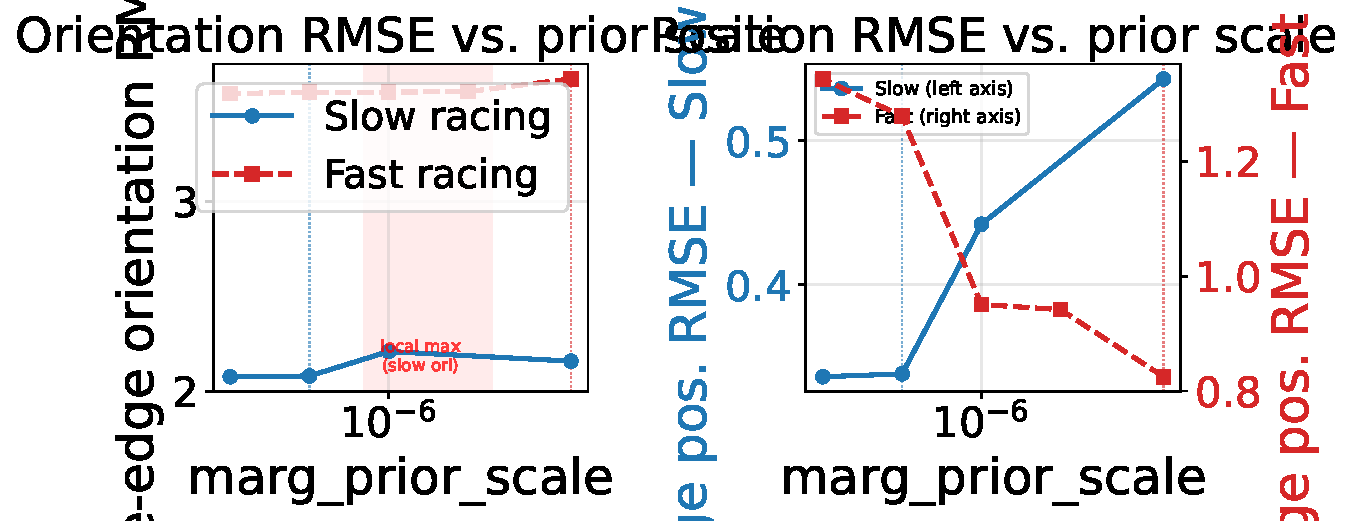
\includegraphics[width=\columnwidth]{figures/prior_scale_sensitivity.pdf}
  \caption{Live-edge orientation (left) and position (right, dual
    y-axes) RMSE vs.\ \texttt{marg\_prior\_scale}.  Orientation
    (left): slow racing shows a local maximum at $10^{-6}$;
    fast racing orientation is insensitive to scale.
    Position (right): slow racing worsens monotonically with
    increasing scale while fast racing improves sharply ---
    the two bags require opposite scale regimes.}
  \label{fig:prior_scale}
\end{figure}

\subsection{Other Negative Results}
\label{sec:negative}

\textbf{IMU preintegration.}
Replacing per-sample gyro/accel factors with Forster
TRO-2017~\cite{forster2017manifold} preintegrated factors at 100\,Hz
reduces constraint density from 8:1 (samples per knot) to 1:1,
degrading orientation RMSE from 1.02\degree\ to 6.40\degree\ and
position RMSE from 0.169\,m to 0.288\,m on slow racing.
The smaller Jacobian yields a faster iteration time,
but the accuracy loss is unacceptable.

\textbf{GNC (Graduated Non-Convexity).}
Geman-McClure loss annealing~\cite{yang2020gnc} was tested on radar
residuals.  It improved results only when extrinsics were incorrect
(masking calibration errors as outliers); with correct calibration it
degraded both bags and added $3\times$ runtime.

\textbf{Full extrinsic optimization.}
The C++ solver only supports the 1-DOF pitch offset $\delta_\text{pitch}$
(Sec.~\ref{sec:state}), because Doppler cannot observe roll or yaw.
When tested in an earlier Python-based solver that allowed all three
angles to optimize freely, roll and yaw drifted 5--7\degree,
using the unobservable modes as a residual trash can and corrupting
orientation by 6--8\degree.  The C++ design avoids this by construction.

%==================================================================
\section{Conclusion}
\label{sec:conclusion}

\emph{Can a single-chip mmWave radar plus IMU provide usable 6-DOF
state estimation?}  Yes --- as a \emph{velocity and orientation}
source: at the live leading edge,
\SI{0.45}{\metre\per\second}/\SI{1.9}{\degree} on gentle racing,
\SI{0.32}{\metre\per\second}/\SI{2.8}{\degree} on aggressive racing
(0.35--0.70\,s per window on a laptop), confirmed on held-out flights
and with NEES-consistent orientation covariance.
Absolute position is not observable from Doppler+IMU and drifts with
distance (0.6--0.9\% on racing, 2.9\% under tumbling); yaw requires a
heading sensor.  Within those structural limits, \emph{good results
took three things}: (1) a \emph{consistent} fixed-lag smoother ---
the Markov-blanket factor-selection rule makes the marginalization a
true marginal, eliminating regime-dependent prior tuning whose
symptom pattern we document as a reusable diagnostic;
(2) a \emph{dynamics-adaptive trust allocation} across the
measurement streams (rate-adaptive gyroscope weight, rate-inflated
radar/accelerometer noise, per-point SNR weighting) --- one
configuration from hover to \SI{10}{\radian\per\second}, with the
velocity--orientation trade made explicit as a measured Pareto curve;
and (3) \emph{characterized sensor systematics} --- including the
finding that the apparent elevation bias under tumbling is a
flight-regime error proxy, not an antenna constant, and that the
extrinsic pitch is a calibration plateau best locked, not estimated
online.  Notably, the largest accuracy gains came from diagnosis-led
re-weighting of existing measurements, not from added model capacity:
a representation-level study showed the orientation spline already
tracks \SI{10}{\radian\per\second} flips at the gyroscope noise floor,
disproving our own adaptive-knot-density hypothesis before
implementation.

Open limitations: (1) loop-scale position geometry through flips is
bounded by during-flip radar data quality (Doppler noise
$15\times$ the level-flight core), demonstrated by an asymmetric
factor-split ablation; (2) ground truth itself degrades during flips
(MoCap occlusion), bounding what can be measured there; and
(3) cross-validation against the EKF-RIO family
(Sec.~\ref{sec:baselines}) reveals a design-space split.  With our
default RANSAC front-end --- the same single-chip outlier rejection
\mbox{reve} uses --- our solver reaches position parity on their public
flights ($0.5$--$1.9$\,m, same order as the baselines), matches their
roll/pitch, and leads on heading-aided orientation; the prefilter is
what closes the single-chip elevation-bias gap, turning a Huber-only
port's $12$--$15\%$ vertical drift into baseline parity.  In the reverse
direction their stock filters, starved by our sparse ${\sim}13$-point
clouds and racing-frame vibration, reject up to 99.7\% of radar updates
and dead-reckon on our slow-racing bag (degrading, not diverging, on the
faster one).  Each stack is engineered for its own regime --- dense
clouds and a low-vibration carrier versus sparse, finely quantized
Doppler on an aggressive platform.

%==================================================================
\bibliographystyle{IEEEtran}
\bibliography{references}

% Author biography (<=100 words; required for the final accepted version,
% optional for initial submission). Replace with degrees/dates as appropriate.
\begin{IEEEbiographynophoto}{Timo Weiss}
is with the Technical University of Munich (TUM), Munich, Germany. His
research interests include radar-inertial odometry, continuous-time
state estimation on Lie groups, and aerial robotics in
perception-degraded conditions.
\end{IEEEbiographynophoto}

\end{document}
